% This is a beamer template created by bingining in Oct 12, 2013.
\documentclass[xcolor={svgnames},compress]{beamer} 
\usepackage[UTF8]{ctex}
\usetheme{Copenhagen}
\usefonttheme{professionalfonts}
\useoutertheme[footline=authortitle,subsection=false]{miniframes}
\setbeamercovered{transparent}
\setbeamercolor{bgcyan}{fg=black,bg=cyan}
\setbeamercolor{bggreen}{fg=black,bg=green}
\setbeamercolor{bgred}{fg=black,bg=red}
\hypersetup{
    colorlinks=true,        % color link
    citecolor=blue,         % cite color
    linkcolor=blue,         % link color
    urlcolor=blue      
}
\addtobeamertemplate{headline}{\hypersetup{linkcolor=.}}{}
\addtobeamertemplate{footline}{\hypersetup{linkcolor=.}}{}

\makeatletter
%\setbeamercolor{section in head/foot}{fg=white}
\setbeamercolor{title in head/foot}{parent=subsection in head/foot}
\setbeamertemplate{footline}
{
    \leavevmode%
    \hbox{%
        \begin{beamercolorbox}[wd=.333333\paperwidth,ht=2.25ex,dp=1ex,center]{author in head/foot}%
            \usebeamerfont{author in head/foot}\insertshortauthor
        \end{beamercolorbox}%
        \begin{beamercolorbox}[wd=.333333\paperwidth,ht=2.25ex,dp=1ex,center]{title in head/foot}%
            \usebeamerfont{title in head/foot}\hypersetup{hidelinks}%
            \insertshorttitle
        \end{beamercolorbox}%
        \begin{beamercolorbox}[wd=.333333\paperwidth,ht=2.25ex,dp=1ex,right]{date in head/foot}%
            \usebeamerfont{date in head/foot}\insertshortdate{}\hspace*{2em}
            \insertframenumber{} / \inserttotalframenumber\hspace*{2ex} 
    \end{beamercolorbox}}%
    \vskip0pt%
}
\makeatother
\beamertemplatenavigationsymbolsempty 
\hypersetup{pdfpagemode=FullScreen} % full-screen when viewing the pdf
\AtBeginSection[]
{
    \begin{frame}<beamer>
        \frametitle{提纲}
        \tableofcontents[currentsection]
    \end{frame}
}
%show a plan before every section
% ajust the vspace on item
\let\olditem\item
\renewcommand{\item}{%
    \olditem\vspace{\fill}}    

\setlength{\tabcolsep}{1pt}
\renewcommand{\arraystretch}{1.3} 

\usepackage[cal=rsfs,scr=euler]{mathalfa}
\usepackage{tabularx}
\usepackage{graphicx} % include graphs
\usepackage{colortbl,amsmath,amssymb}
\usepackage{textpos} % add logo
\usepackage{tensor} % manipulate tensor
\usepackage[most]{tcolorbox} % equation array box
\usepackage{multirow}


%%%%%%%%%%%%%%%%%%%%%%%%%%%%%%%%%%%%%%%%%%%%%%%%%%%%%%%%%%%%%%%%%%%%%%
% newcommand % 
%%%%%%%%%%%%%%%%%%%%%%%%%%%%%%%%%%%%%%%%%%%%%%%%%%%%%%%%%%%%%%%%%%%%%%
\usepackage{tensor}     % manipulate tensors
\usepackage{graphicx}   % include figures
\graphicspath{{Img/}} %Setting the graphicspath 
%\usepackage{bm}         % \bm{<text>} Bold math symbols
\usepackage{xcolor}     % textcolor
%\usepackage{cancel}     % slashes in equtions
%\usepackage{ulem}     % underline of equations
\usepackage{amsmath}	% AMS Math Package
\usepackage{amsthm}	% Theorem Formatting
\usepackage{amssymb}
\usepackage{datetime}
\usepackage{graphicx}
\usepackage{color}
%\usepackage{verbatim}
\usepackage{float}
%\usepackage{bm}

\newcommand{\nc}{\newcommand*}
\nc{\newc}{\newcommand}
\nc{\bm}[1]{\mathbf{#1}}
\nc{\figurewidth}{3.2in}
\nc{\xbar}{\bar{x}}
\nc{\rhoeq}{\rho_{\rm{eq}}}
\nc{\zeq}{z_{\rm{eq}}}
\nc{\la}{\lambda}
\nc{\tla}{\tilde{\la}}
\nc{\dt}{\delta}
\nc{\Dt}{\Delta}
\nc{\vj}{\vec{j}}
\nc{\vl}{\vec{l}}
\nc{\hx}{\hat{x}}
\nc{\hy}{\hat{y}}
\nc{\bj}{\mathbf{j}}
\nc{\mJ}{\mathcal{J}}
\nc{\mP}{\mathcal{P}}
\nc{\ga}{\gamma}
\nc{\Msun}{M_\odot}
\nc{\app}{\approx}
\nc{\av}[1]{\langle #1 \rangle}
\nc{\eq}[1]{Eq.~\eqref{#1}}
\nc{\al}{\alpha}
\nc{\Xstar}{X_{\ast}}
\nc{\seq}{\sigma_{\rm{eq}}}
\nc{\fpbh}{f_{\mathrm{PBH}}}
\nc{\VT}{\langle VT \rangle}


\nc{\s}{\sigma}
\nc{\Ld}{\Lambda}
\nc{\p}{\partial}
\nc{\Om}{\Omega}
\nc{\rd}{\mathrm{d}}
\nc{\Od}{\mathcal{O}}

%\nc{\ld}{\lambda}
%\nc{\gm}{\gamma}
\nc{\vth}{\vec{\theta}}
\nc{\vla}{\vec{\lambda}}
\nc{\vd}{\vec{d}}
\nc{\Mmin}{M_{\mathrm{min}}}
\nc{\rmd}{\mathrm{d}}
\nc{\mmin}{{m_{\mathrm{min}}}}
\nc{\mmax}{{m_{\mathrm{max}}}}
\nc{\mR}{\mathcal{R}}
\nc{\tmR}{\tilde{\mathcal{R}}}
\nc{\ogw}{\Omega_{\mathrm{GW}}}
\nc{\addref}{[\textcolor{red}{add ref}] }
\nc{\gpcyr}{\mathrm{Gpc}^{-3}\,\mathrm{yr}^{-1}}
\nc{\Eq}[1]{公式\eqref{#1}}
\nc{\Fig}[1]{图\ref{#1}}
\nc{\Table}[1]{表\ref{#1}}
\nc{\lvc}{LIGO-Virgo} % LIGO-VIRGO collaboration
\nc{\Sec}[1]{Sec.~\ref{#1}}
\nc{\eg}{\textit{e.g.~}}
\nc{\SNR}{\mathrm{SNR}}
\nc{\fpbhn}{f_{\mathrm{PBH0}}}    % f_pbh
\nc{\fmin}{{f_{\mathrm{min}}}}
\nc{\rhoGW}{\rho_{\mathrm{GW}}}
\nc{\Nobs}{N_{\mathrm{obs}}}
\nc{\km}{\mathrm{km}}
\nc{\Mpc}{\mathrm{Mpc}}
\nc{\Tobs}{T_{\mathrm{obs}}}
\nc{\Ntemp}{N_{\mathrm{temp}}}

\nc{\mH}{\mathcal{H}}
\nc{\cs}{c_s^2}
\nc{\Sij}[1]{S_{ij}^{(#1)}}
\nc{\vi}[1]{v_i^{(#1)}}
\nc{\no}{\nonumber}
\def\<{\left\langle}
\def\>{\right\rangle}
\def\ap{\alpha}
\def\half{{1\over 2}}
\nc{\bk}{\bm{k}}
\nc{\bq}{\bm{q}}
\nc{\bp}{\bm{p}}
\nc{\bl}{\bm{l}}
\nc{\bx}{\bm{x}}
\nc{\be}{\mathbf{e}}
\nc{\mS}{\mathcal{S}}
\nc{\te}{\tilde{\eta}}
\nc{\tp}{\tilde{p}}
\nc{\tk}{\tilde{k}}
\nc{\tx}{\tilde{x}}
\nc{\tF}{\tilde{F}}
\nc{\tA}{\tilde{A}}
\nc{\mkpq}{|\bk-\bp-\bq|}
\nc{\mpq}{|\bp-\bq|}
\nc{\mkp}{|\bk-\bp|}
\nc{\mSi}[1]{\mS^{(#1)}({\bk, \eta})}
\nc{\vk}{\vec{k}}
\nc{\kstar}{k_*}
\nc{\fstar}{f_*}
\nc{\xstar}{x_*}
\nc{\mpbh}{m_{\rm{pbh}}}
\nc{\bn}[1]{\dt\bm{t}_{\text{#1}}}
\nc{\bC}[1]{\bm{C}_{\text{#1}}}
\nc{\NTOA}{N_{\text{TOA}}}
\nc{\Nmode}{{N_{\text{mode}}}}
\nc{\ARN}{A_{\rm{RN}}}
\nc{\gRN}{\gamma_{\rm{RN}}}
\nc{\bS}{\mathbf{\Sigma}}
\nc{\br}{\mathbf{r}}
\nc{\bN}{\mathbf{R}}
\nc{\TTT}{\mathrm{TT}}

%%%%%%%%%%%%%%%%%%%%%%%%%%% greek letters %%%%%%%%%%%%%%%%%%%%%%%%%%%%
\newc{\zt}{\zeta}
\newc{\et}{\eta}
\newc{\ta}{\theta}
\newc{\io}{\iota}
\newc{\kp}{\kappa}
\newc{\La}{\Lambda}
\newc{\oo}{\omicron}
\newc{\sg}{\sigma}
\newc{\Sg}{\Sigma}
\newc{\om}{\omega}
\newc{\vp}{\varphi}
\newc{\Ga}{\Gamma}

%%%%%%%%%%%%%%%%%%%%%%%%%%%%%%% fonts %%%%%%%%%%%%%%%%%%%%%%%%%%%%%%%%
\newc{\mc}{\mathcal}
\newc{\ms}{\mathscr}
\newc{\mb}{\mathbf} 
\newc{\ie}{\textit{i.e. }}
\newc{\etc}{\textit{etc. }}
\newc{\etal}{\textit{et al. }}
\newc{\lcdm}{$\Lambda$CDM}
\newc{\gs}{\sqrt{-g}}

%%%%%%%%%%%%%%%%%%%%%%%%%%%%% other %%%%%%%%%%%%%%%%%%%%%%%%%%%%%%%%%%
\newc{\ts}{\tensor}
\newc{\td}{\tilde}
\newc{\hf}{\frac{1}{2}}
\newc{\ra}{\rightarrow}
\newc{\Ra}{\Rightarrow}
\newc{\lra}{\leftrightarrow}
\newc{\Lra}{\Leftrightarrow}
\newc{\so}{\therefore}
\newc{\nb}{\nabla}
\newc{\LA}{\mathop{}\!\mathbin\bigtriangleup} %Laplace
\newc{\DA}{\mathop{}\!\mathbin\Box} %DAlambert
\newc{\lp}{\left(} % left parenthesis
\newc{\rp}{\right)} % right parenthesis
\newc{\lb}{\left[} % left bracket
\newc{\rb}{\right]} % right bracket
\newc{\lB}{\left\{} % left Brace
\newc{\rB}{\right\}} % right Brace
\newc{\ef}{Eq.\eqref}
\newc{\red}[1]{\textcolor{red}{#1}}
\newc{\add}{\red{\emph{(add some comments or explanations)}\\}}
%%%%%%%%%%%%%%%%%%%%%% only used in this file %%%%%%%%%%%%%%%%%%%%%%%%
\newc{\Td}[1]{ \ts{\dt}{#1} }
\newc{\Th}[1]{\ts{h}{#1}} % tesor h
\newc{\h}[1]{\ts{\bar{h}}{#1}} % trace-reverse tensor
\newc{\Tg}[1]{\ts{\ga}{#1}}
\newc{\TG}[1]{\ts{\Ga}{#1}} % tensor \Gamma
\newc{\Bg}{\bm{g}}
\newc{\Bf}{\bm{f}}
\newc{\BG}{\bm{\ga}}
\newc{\tr}[1]{\lb #1 \rb}
\newc{\gts}{ \sqrt{-\td{g}}}
\newc{\nt}[1]{\ts{\td{\nabla}}{#1}}
\newc{\da}{\td{\DA}}
\newc{\tn}{\td{\nb}}
\newc{\Gone}[1]{\overset{1}{\Ga}\ts{}{#1}} 
\newc{\Gtwo}[1]{\overset{2}{\Ga}\ts{}{#1}}
\newc{\Etwo}[1]{\overset{2}{G}\ts{}{#1}} % second order of Einstein tensor 
\newc{\Rone}[1]{\overset{1}{R}\ts{}{#1}} 
\newc{\Rtwo}[1]{\overset{2}{R}\ts{}{#1}} 
%\newc{\TT}{\overset{TT}{=}} 
\nc{\TT}{\mathrm{TT}}
\newc{\hone}[1]{\overset{1}{h}\ts{}{#1}} 
\newc{\htwo}[1]{\overset{2}{h}\ts{}{#1}} 
\newcommand{\order}[1]{\mathcal{O}\left(#1\right)}
\newcommand{\avg}[1]{\left \langle #1 \right \rangle}
\nc{\GW}{\mathrm{GW}}
%%%%%%%%%%%%%%%%%%%%%%%%%%%%%%%%%%%% other %%%%%%%%%%%%%%%%%%%%%%%%%%%%%%%%%%%%
\def\half{{1\over 2}}

\def\p{\partial}
\def\ap{\alpha'}
\def\({\left(}
\def\){\right)}
\def\Mpl{M_{\rm P}}


%%%%%%%%%%%%%%%%%%%%%%%%%%%%%%%%%%% equations %%%%%%%%%%%%%%%%%%%%%%%%%%%%%%%%%%
\def\({\left(}
\def\){\right)}
\def\e{\begin{equation}}
\def\q{\end{equation}}
\def\m{\begin{eqnarray}}
\def\n{\end{eqnarray}}
\nc{\blue}[1]{\textcolor{blue}{#1}}
\nc{\Refs}[1]{{\tiny{\textcolor{blue}{\textit{#1}}}}}
%%%%%%%%%%%%%%%%%%%%%%%%%%%%%%%%%%%%%%%%%%%%%%%%%%%%%%%%%%%%%%%%%%%%%%%%%%%%%%%%
%%%%%%%%%%%%%%%%%%%%%%%%%%%%%%%%%%%%%%%%%%%%%%%%%%%%%%%%%%%%%%%%%%%%%%


%%%%%%%%%%%%%%%%%%%%%%%%%%%%%%%%%%%%%%%%%%%%%%%%%%%%%%%%%%%%%%%%%%%%%%%%%%%%%%%%
\begin{document}

\kaishu

%%%%%%%%%%%%%%%%%%%%%%%%%%%%%%%%%%%%%%%%%%%%%%%%%%%%%%%%%%%%%%%%%%%%%%
% add logo on every frame
\addtobeamertemplate{frametitle}{}{%
    \begin{textblock*}{50mm}(0.98\textwidth,-8.5mm)
        
\includegraphics[height=7mm,width=7mm]{./Img/cas_logo}
    \end{textblock*}
}
%%%%%%%%%%%%%%%%%%%%%%%%%%%%%%%%%%%%%%%%%%%%%%%%%%%%%%%%%%%%%%%%%%%%%%
% title page 
%%%%%%%%%%%%%%%%%%%%%%%%%%%%%%%%%%%%%%%%%%%%%%%%%%%%%%%%%%%%%%%%%%%%%%
\title{通过引力波探测原初黑洞}
\author[陈祖成]{\Large 报告人:陈祖成
    \\ 导\quad 师: 黄庆国}

%\date{\today}
\date{2021年5月20日}

\institute{\large 中国科学院理论物理研究所}

\titlegraphic{

\includegraphics[width=0.7\columnwidth]{./Img/ucas_logo}\quad

\includegraphics[width=0.16\columnwidth]{./Img/itp_logo.jpg}
}

%%%%%%%%%%%%%%%%%%%%%%%%%%%%%%%%%%%%%%%%%%%%%%%%%%%%%%%%%%%%%%%%%%%%%%
\begin{frame}[plain]
\titlepage
\end{frame}


\begin{frame}{引力波相关文章}
    \vspace{-2mm}
    \begin{enumerate}
        \item \href{https://journals.aps.org/prd/abstract/10.1103/PhysRevD.100.081301}{Probing primordial-black-hole dark matter with scalar induced gravitational waves} \\
        Phys.Rev.D 100 (2019) 8, 081301\\
        Chen Yuan, \textbf{Zu-Cheng Chen}, Qing-Guo Huang    
        
        \item \href{https://link.springer.com/article/10.1007/s11433-019-9605-5}{Measuring the tilt of primordial gravitational-wave power spectrum from observations}\\
        Sci.China Phys.Mech.Astron. 62 (2019) 11, 110421\\
        Jun Li, \textbf{Zu-Cheng Chen}, Qing-Guo Huang
        
        \item \href{https://journals.aps.org/prd/abstract/10.1103/PhysRevD.101.043019}{Log-dependent slope of scalar induced gravitational waves in the infrared regions}\\
            Phys.Rev.D 101 (2020) 4, 043019\\ 
        Chen Yuan, \textbf{Zu-Cheng Chen}, Qing-Guo Huang    
          
        
    \end{enumerate} 
\end{frame}

%%%%%%%%%%%%%%%%%%%%%%%%%%%%%%%%%%%%%%%%%%%%%%%%%%%%%%%%%%%%%%%%%%%%%%%%%%%%%%%%
\begin{frame}{引力波相关文章}
    \begin{enumerate}   
        \setcounter{enumi}{3} 
        \item \href{https://link.springer.com/article/10.1007\%2Fs11467-019-0936-x}{Extraction of gravitational wave signals with optimized convolutional neural network}\\
        Front.Phys.(Beijing) 15 (2020) 1, 14601\\
        Hua-Mei Luo, Wenbin Lin, \textbf{Zu-Cheng Chen}, Qing-Guo Huang  
        
        \item \href{https://journals.aps.org/prd/abstract/10.1103/PhysRevD.101.063018}{Scalar induced gravitational waves in different gauges}\\
        Phys.Rev.D 101 (2020) 6, 063018\\
        Chen Yuan, \textbf{Zu-Cheng Chen}, Qing-Guo Huang
        
        \item \href{https://arxiv.org/abs/2101.06869}{Non-tensorial Gravitational Wave Background in NANOGrav 12.5-Year Data Set}\\ \href{https://arxiv.org/abs/2101.06869}{arXiv:2101.06869 [astro-ph.CO]}\\
        \textbf{Zu-Cheng Chen}, Chen Yuan, Qing-Guo Huang
        %
    \end{enumerate} 
\end{frame}
%%%%%%%%%%%%%%%%%%%%%%%%%%%%%%%%%%%%%%%%%%%%%%%%%%%%%%%%%%%%%%%%%%%%%%

%%%%%%%%%%%%%%%%%%%%%%%%%%%%%%%%%%%%%%%%%%%%%%%%%%%%%%%%%%%%%%%%%%%%%%
\begin{frame}{原初黑洞相关文章}
    \vspace{-2mm}
    \begin{enumerate}
        \item \href{https://iopscience.iop.org/article/10.3847/1538-4357/aad6e2}{Merger Rate Distribution of Primordial-Black-Hole Binaries}\\
        Astrophys.J. 864 (2018) 1, 61\\
        \textbf{Zu-Cheng Chen},Qing-Guo Huang
        
        \item \href{https://iopscience.iop.org/article/10.3847/1538-4357/aaf581}{Stochastic Gravitational-Wave Background from Binary Black Holes and Binary Neutron Stars and Implications for LISA}\\
        Astrophys.J. 871 (2019) 1, 97\\
        \textbf{Zu-Cheng Chen}, Fan Huang, Qing-Guo Huang
        
        \item \href{https://iopscience.iop.org/article/10.1088/1475-7516/2020/08/039}{Distinguishing Primordial Black Holes from Astrophysical Black Holes by Einstein Telescope and Cosmic Explorer}\\
        JCAP 08 (2020) 039\\
        \textbf{Zu-Cheng Chen},Qing-Guo Huang
        
        \item \href{https://journals.aps.org/prl/abstract/10.1103/PhysRevLett.124.251101}{Pulsar Timing Array Constraints on Primordial Black Holes with NANOGrav 11-Year Dataset}\\
        Phys.Rev.Lett. 124 (2020) 25, 251101\\    
        \textbf{Zu-Cheng Chen}, Chen Yuan, Qing-Guo Huang 
        
    \end{enumerate} 
\end{frame}
%%%%%%%%%%%%%%%%%%%%%%%%%%%%%%%%%%%%%%%%%%%%%%%%%%%%%%%%%%%%%%%%%%%%%%
% contents
%%%%%%%%%%%%%%%%%%%%%%%%%%%%%%%%%%%%%%%%%%%%%%%%%%%%%%%%%%%%%%%%%%%%%%
\begin{frame}{提纲}
    %    \setcounter{tocdepth}{1}
    \tableofcontents
\end{frame}

%%%%%%%%%%%%%%%%%%%%%%%%%%%%%%%%%%%%%%%%%%%%%%%%%%%%%%%%%%%%%%%%%%%%%%
\section{引言}
\subsection{}
%%%%%%%%%%%%%%%%%%%%%%%%%%%%%%%%%%%%%%%%%%%%%%%%%%%%%%%%%%%%%%%%%%%%%%
\begin{frame}{}
    \centering
    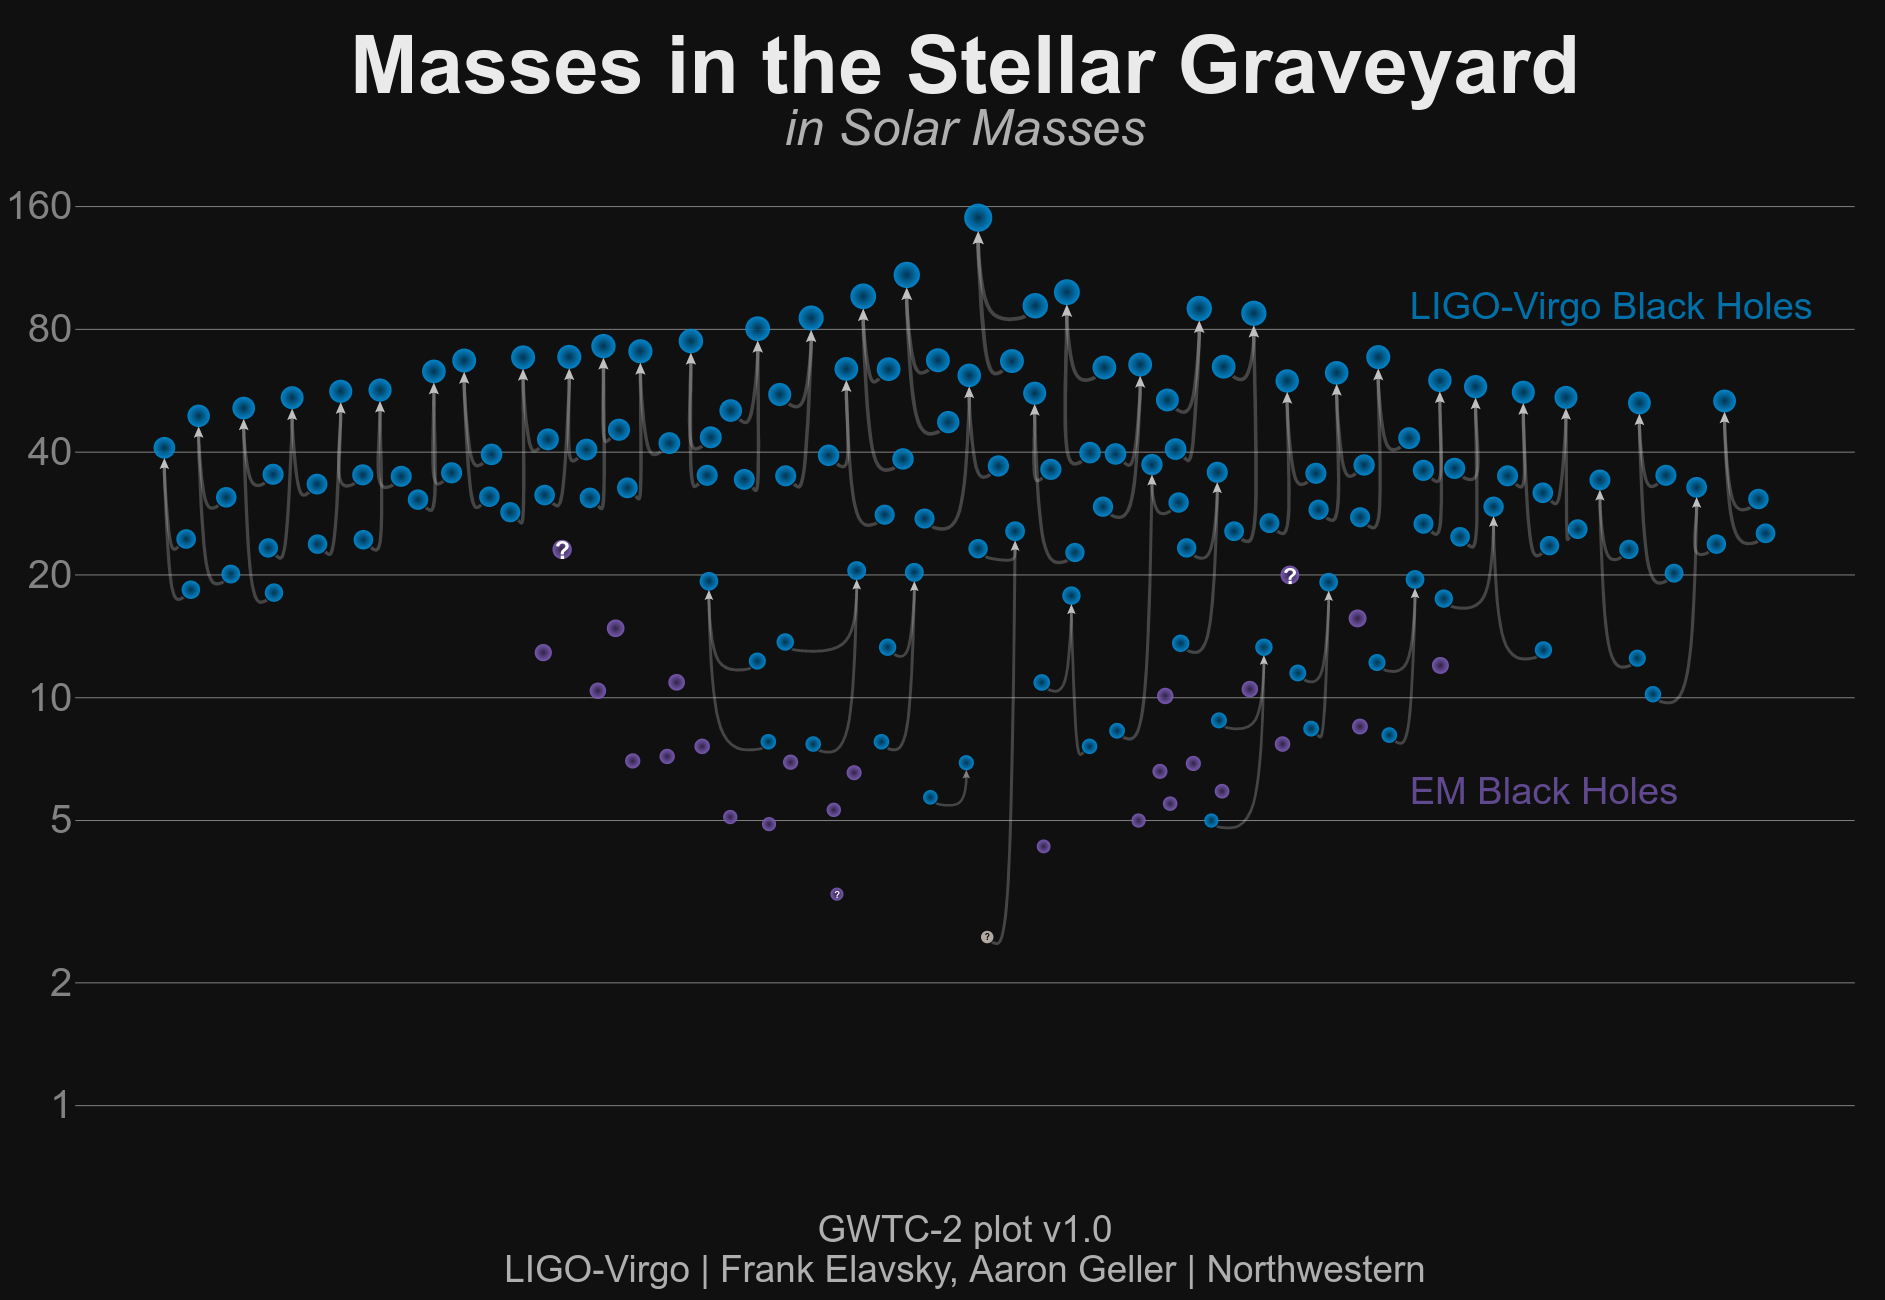
\includegraphics[width=\textwidth]{Masses_of_Dead_Stars_LIGO_Virgo}
\end{frame}
%%%%%%%%%%%%%%%%%%%%%%%%%%%%%%%%%%%%%%%%%%%%%%%%%%%%%%%%%%%%%%%%%%%%%%


%%%%%%%%%%%%%%%%%%%%%%%%%%%%%%%%%%%%%%%%%%%%%%%%%%%%%%%%%%%%%%%%%%%%%%
\begin{frame}{}
    \begin{block}{\lvc 的引力波探测告诉我们}
        \begin{itemize}
            \vspace{2mm}
            \item 宇宙中有很多双黑洞(BBH)。
            \item 这些双黑洞可以在哈勃时间内并合。
            \item 黑洞是有质量分布的。 
        \end{itemize}
    \end{block}
%    \pause
    \begin{alertblock}{未解之谜}
        \begin{itemize}
            \vspace{2mm}
            \item 这些黑洞的起源是什么?
            \item 以及是如何成对的?
            \item 为什么引力波探测到的黑洞的质量要比X射线探测到的黑洞的质量大很多?
        \end{itemize}
    \end{alertblock}
\centering
一个可能的解释是原初黑洞。
\end{frame}
%%%%%%%%%%%%%%%%%%%%%%%%%%%%%%%%%%%%%%%%%%%%%%%%%%%%%%%%%%%%%%%%%%%%%%


%%%%%%%%%%%%%%%%%%%%%%%%%%%%%%%%%%%%%%%%%%%%%%%%%%%%%%%%%%%%%%%%%%%%%%
\begin{frame}{原初黑洞(Primordial Black Hole, PBH)}
    \vspace{-3mm}
    \begin{columns}
        \begin{column}{0.7\textwidth}
            \begin{itemize}
                \item 原初黑洞是在宇宙早期由于原初密度扰动坍塌而形成的黑洞。
                \Refs{Mon.Not.Roy.Astron.Soc. 152 (1971) 75}
                \item 原初黑洞的质量可以跨越很多个数量级
                \e 
                m_{\mathrm{PBH}} \sim \frac{t}{G} \sim 10^{-18} 
                \left(
                \frac{t}{10^{-23}}
                \right) \Msun
                \q
                \item 未蒸发掉的原初黑洞可以作为暗物质的候选者。
                \item 原初黑洞可以解释\lvc 探测到的黑洞。
            \end{itemize}
        \end{column}
        \begin{column}{0.4\textwidth} 
            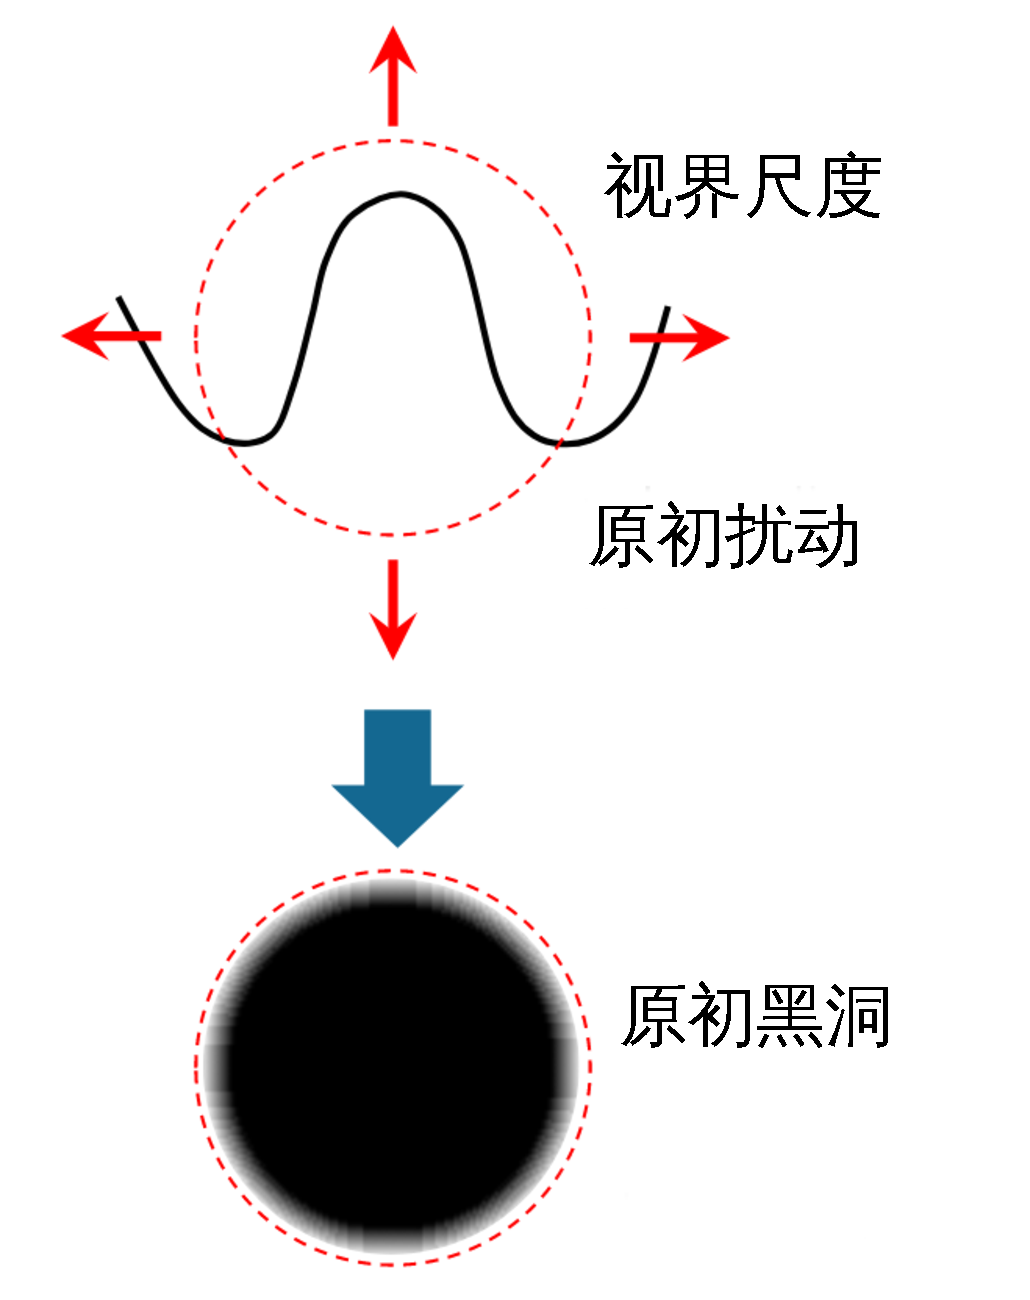
\includegraphics[width=\textwidth]{pbh_form} 
        \end{column}
    \end{columns}
    \vspace{2mm}
%             
\end{frame}
%%%%%%%%%%%%%%%%%%%%%%%%%%%%%%%%%%%%%%%%%%%%%%%%%%%%%%%%%%%%%%%%%%%%%%

\section{原初双黑洞的并合率}
\subsection{}
%%%%%%%%%%%%%%%%%%%%%%%%%%%%%%%%%%%%%%%%%%%%%%%%%%%%%%%%%%%%%%%%%%%%%%
\begin{frame}{研究动机}
    \begin{itemize}
        \item 为了解释引力波探测到的双黑洞,需要知道原初双黑洞的并合率分布。
        \item 引力波探测到的黑洞是有质量分布的。
        \item 考虑任意的原初黑洞的质量谱$P(m)$
        {\small
        \[
        \int P(m)dm=1.
        \]
    }
        \centering
        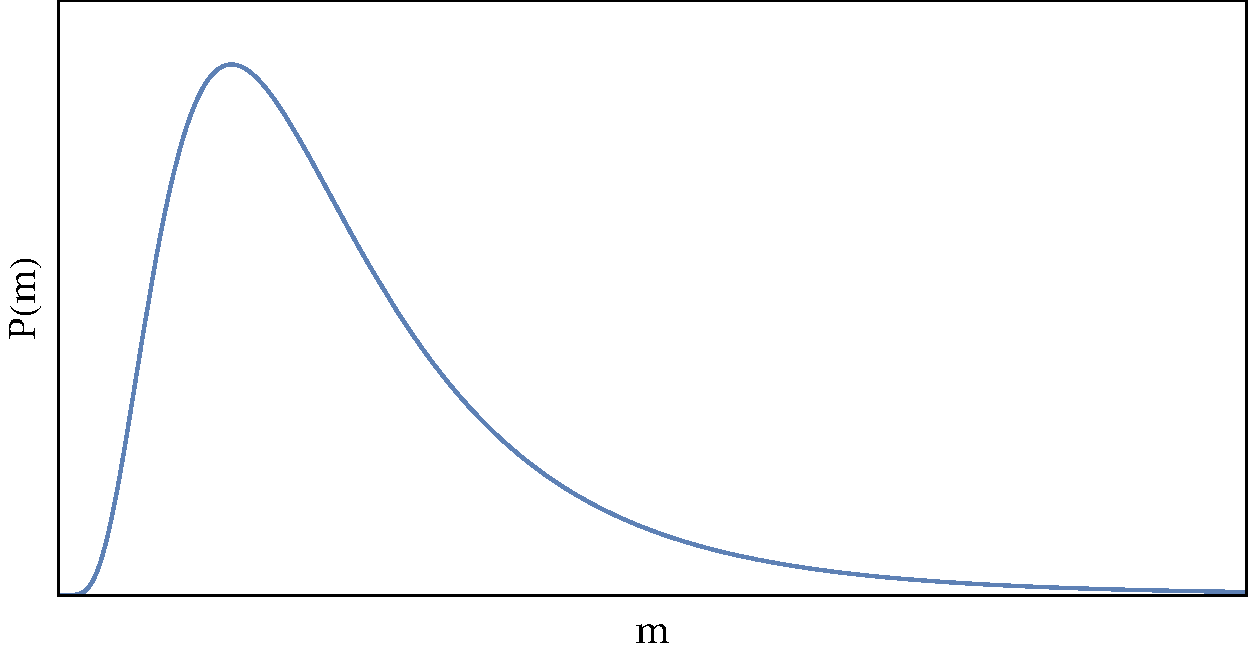
\includegraphics[width=0.7\textwidth]{pm} 
    \end{itemize}
\end{frame}
%%%%%%%%%%%%%%%%%%%%%%%%%%%%%%%%%%%%%%%%%%%%%%%%%%%%%%%%%%%%%%%%%%%%%%


%%%%%%%%%%%%%%%%%%%%%%%%%%%%%%%%%%%%%%%%%%%%%%%%%%%%%%%%%%%%%%%%%%%%%%
\begin{frame}{小结}	
    \begin{itemize}        
        \item 计算了原初黑洞具有一般质量谱时,原初双黑洞的并合率分布。
        \item 证实原初黑洞可以解释\lvc 探测到的双黑洞事件。
        \item 证实绝大多数的冷暗物质不是由恒星级质量的原初黑洞构成的。
    \end{itemize}
\end{frame}
%%%%%%%%%%%%%%%%%%%%%%%%%%%%%%%%%%%%%%%%%%%%%%%%%%%%%%%%%%%%%%%%%%%%%%

%%%%%%%%%%%%%%%%%%%%%%%%%%%%%%%%%%%%%%%%%%%%%%%%%%%%%%%%%%%%%%%%%%%%%%

\section{原初双黑洞产生的引力波背景}
\subsection{}
%%%%%%%%%%%%%%%%%%%%%%%%%%%%%%%%%%%%%%%%%%%%%%%%%%%%%%%%%%%%%%%%%%%%%%
\begin{frame}{研究动机}
    \begin{itemize}
        \item \lvc 目前只能探测到红移$z\lesssim 2$的双黑洞并合事件。
        \item 所有双黑洞并合产生的引力波信号会叠加形成随机引力波背景。
        \item 除了探测单个原初双黑洞产生的引力波外,还可以探测原初双黑洞产生的随机引力波背景。
    \end{itemize}
\end{frame}
%%%%%%%%%%%%%%%%%%%%%%%%%%%%%%%%%%%%%%%%%%%%%%%%%%%%%%%%%%%%%%%%%%%%%%


%%%%%%%%%%%%%%%%%%%%%%%%%%%%%%%%%%%%%%%%%%%%%%%%%%%%%%%%%%%%%%%%%%%%%%
\begin{frame}{小结}	
    \begin{itemize}        
        \item 计算了原初双黑洞产生的随机引力波背景。
        \item 此引力波背景可以被LIGO设计阶段和LISA探测到。
        \item 如果此引力波背景没能从LISA的噪音中扣除掉,将会构成LISA的额外噪音,从而降低LISA的探测能力。
    \end{itemize}
\end{frame}
%%%%%%%%%%%%%%%%%%%%%%%%%%%%%%%%%%%%%%%%%%%%%%%%%%%%%%%%%%%%%%%%%%%%%%

\section{总结}
%%%%%%%%%%%%%%%%%%%%%%%%%%%%%%%%%%%%%%%%%%%%%%%%%%%%%%%%%%%%%%%%%%%%%%
\begin{frame}{总结}
    \begin{itemize}
        \item 计算原初黑洞具有一般质量谱时,原初双黑洞的并合率分布;证实恒星级质量的原初黑洞无法构成绝大部分冷暗物质。
        
        \item 计算了原初双黑洞产生的随机引力波背景,并发现此背景可以被LISA探测到。如果此背景没能从LISA噪音中扣除掉,将会构成LISA的额外噪音,从而降低LISA的探测能力。
        
        \item 探讨如何通过ET和CE来区分原初黑洞和天体物理黑洞。通过定向搜寻包含至少一个亚太阳质量黑洞的双黑洞系统,估算了$\fpbh$的可探测极限。并预测了ET和CE能够探测到的双黑洞事件数目随红移的分布,从而来区分原初黑洞和天体物理黑洞。
        
        \item 在NANOGrav 11年的数据中搜寻伴随原初黑洞形成而产生的标量诱导引力波。由于没有发现引力波信号,所以在$0.002\sim 0.7\Msun$的质量区间,$\fpbh < 10^{-6}$。
    \end{itemize}  
\end{frame}

%%%%%%%%%%%%%%%%%%%%%%%%%%%%%%%%%%%%%%%%%%%%%%%%%%%%%%%%%%%%%%%%%%%%%%
\begin{frame}{展望}
    \begin{itemize}
        \item 用\lvc 最新的数据GWTC-2来重构原初黑洞质量谱$P(m)$以及拟合原初黑洞模型。
        
        \item 考虑原初黑洞和天体物理黑洞同时存在的情况。
        
        \item 在NANOGrav 12.5年的数据中搜索引力波信号:
        \begin{itemize}
            \item 标量诱导引力波
            \item 其它极化模式的引力波
        \end{itemize}
    \end{itemize}  
\end{frame}

%%%%%%%%%%%%%%%%%%%%%%%%%%%%%%%%%%%%%%%%%%%%%%%%%%%%%%%%%%%%%%%%%%%%%%
\begin{frame}[plain]
    \begin{center}
        \font\endfont = cmss20 at 25.40mm
        \color{Blue}
        \endfont
        \baselineskip 20.0mm
        \fontsize{50.0pt}{\baselineskip}\selectfont  谢谢!
    \end{center} 
\end{frame}
%%%%%%%%%%%%%%%%%%%%%%%%%%%%%%%%%%%%%%%%%%%%%%%%%%%%%%%%%%%%%%%%%%%%%%
%%%%%%%%%%%%%%%%%%%%%%%%%%%%%%%%%%%%%%%%%%%%%%%%%%%%%%%%%%%%%%%%%%%%%%
\end{document}
